\documentclass[12pt,compress,ngerman]{beamer}
\usepackage{amsmath}
\usepackage{url}
\usepackage{ucs}
\usepackage[utf8x]{inputenc}
\usepackage[ngerman]{babel}
\usepackage{ulem}  % sout
\usepackage{multicol}

% Manual syntax highlighting
\newcommand{\synfunc}   [1]{\color{blue!50!black}#1\color{black}}
\newcommand{\synstr}    [1]{\color{red!50!black}#1\color{black}}
\newcommand{\synvar}    [1]{\color{purple!50!black}#1\color{black}}
\newcommand{\synclass}  [1]{\color{green!50!black}#1\color{black}}
\newcommand{\syncomment}[1]{\color{blue!20!black}#1\color{black}}
\newcommand{\syncool}   [1]{\color{beamer@blendedblue}#1\color{black}}
\newcommand{\synoder}      {\ \ \color{black}$\vee$\ \ }
\newcommand{\hr}        {\rule[4pt]{\textwidth}{0.1pt}\\}
\newcommand{\hicolor}   [1]{\color[rgb]{0.6,0.2,0.8}#1\color{black}}
\newcommand{\synhilight}[1]{\hicolor{\textbf{#1}}}

\newcommand{\synType}   [1]{\color{red!38!black}#1\color{black}}
\newcommand{\synSym}    [1]{\color{blue!56!black}#1\color{black}}
\newcommand{\synKey}    [1]{\color{blue!56!black}#1\color{black}}
\newcommand{\synLit}    [1]{\color{green!19!black}#1\color{black}}
\newcommand{\synOp}     [1]{\color{green!38!black}#1\color{black}}

\newcommand{\doofcomment}{\ \ \syncomment{\# :-(}}
\newcommand{\gutcomment} {\ \ \syncomment{\# :)}}

\newcommand{\T}[1]{\mathbf{#1}}
\newcommand{\Spur}[1]{\operatorname{Spur}{#1}}
\newcommand{\ul}[1]{\mathcal{#1}}

\definecolor{backblue}{rgb}{0.84,0.84,0.94}
\definecolor{backgrey}{rgb}{0.84,0.84,0.84}

\newcommand{\floatbox}[3]{%
  \raisebox{0pt}[0pt][0pt]{%
    \begin{picture}(0,0)(#1,#2)#3\end{picture}%
  }%
}

\title{Haskell, \\eine rein funktionale Programmiersprache}
\author{Ingo Blechschmidt \\ \texttt{<iblech@web.de>}}
\date{Augsburger Linux-Infotag \\ 27. März 2010}

\usetheme{Warsaw}  %Warsaw, Berkeley?
\usecolortheme{seahorse}
\usefonttheme{serif}
\useinnertheme{rectangles}
\usepackage{bookman}
\setbeamercovered{invisible}

\setbeamertemplate{navigation symbols}{}
%\setbeamertemplate{headline}{}

\begin{document}

\logo{\begin{picture}(0,0)(80,0)
\includegraphics[scale=0.4]{images/haskell-logo.png}\end{picture}}
\frame{\titlepage}
\logo{}

\frame[plain]{\begin{center}
  
\includegraphics[scale=0.35]{images/learn-you-a-haskell-for-great-good.png}
\end{center}}

\frame[t]{\begin{multicols}{2}\tableofcontents\end{multicols}}

\section{Grundlegendes}
\frame[t]{\frametitle{Haskell ist komisch!}
  \floatbox{-210}{110}{
\includegraphics[scale=0.2]{images/endo.png}}%
  Haskell ist rein funktional:
  \begin{itemize}
    \item keine veränderliche Variablen
    \item keine Nebeneffekte
    \item keine Anweisungen
  \end{itemize}
}

\subsection[Variablen]{Keine Variablen}
\frame[t]{\frametitle{Keine veränderliche Variablen}
  \floatbox{-260}{180}{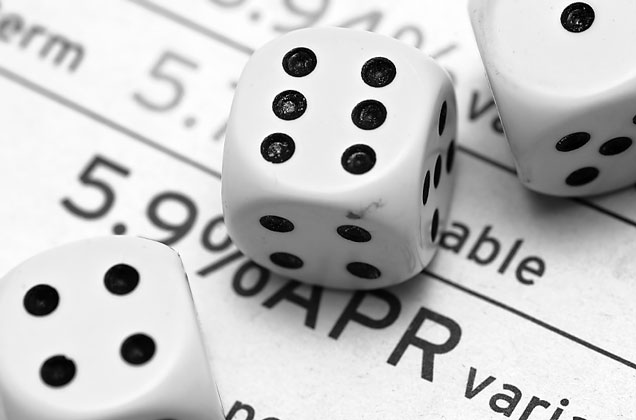
\includegraphics[scale=0.1]{images/variable.jpg}}%
  \texttt{%
    \syncomment{\# Perl} \\
    \synfunc{sub}\ main \{\\
    \ \ \ \ \synfunc{my}\ \synvar{\$radius}\ \ \ \ = 42; \\
    \ \ \ \ \synfunc{my}\ \synvar{\$quadriert}\ = \synvar{\$radius}\ ** 2; \\
    \ \ \ \ \synfunc{my}\ \synvar{\$flaeche}\ \ \ = \synvar{\$quadriert}\ * pi; \\
    \ \ \ \ \synfunc{print}\ \synvar{\$flaeche}; \\
    \}
  }
  \vfill

  \only<2>{
    \texttt{%
      \syncomment{-- Haskell} \\
      main =\\
      \ \ \ \ \synKey{let}\ radius\ \ \ \ \synSym{=}\ \synLit{42} \\
      \ \ \ \ \ \ \ \ quadriert \synSym{=}\ radius\synOp{\^{}}\synLit{2} \\
      \ \ \ \ \ \ \ \ flaeche\ \ \ \synSym{=}\ quadriert \synOp{*}\ pi \\
      \ \ \ \ \synKey{in}\ print\ flaeche
    }
  }

  \only<3>{
    \texttt{%
      \syncomment{-- Haskell} \\
      main =\\
      \ \ \ \ \synKey{let}\ flaeche\ \ \ \synSym{=}\ quadriert \synOp{*}\ pi \\
      \ \ \ \ \ \ \ \ quadriert \synSym{=}\ radius\synOp{\^{}}\synLit{2} \\
      \ \ \ \ \ \ \ \ radius\ \ \ \ \synSym{=}\ \synLit{42} \\
      \ \ \ \ \synKey{in}\ print\ flaeche
    }
  }

  \only<4>{
    \texttt{%
      \syncomment{-- Haskell} \\
      main = print\ flaeche \\
      \ \ \ \ \synKey{where} \\
      \ \ \ \ flaeche\ \ \ \synSym{=}\ quadriert \synOp{*}\ pi \\
      \ \ \ \ quadriert \synSym{=}\ radius\synOp{\^{}}\synLit{2} \\
      \ \ \ \ radius\ \ \ \ \synSym{=}\ \synLit{42}
    }
  }
}

\subsection[Nebeneffekte]{Keine Nebeneffekte}
\frame[t]{\frametitle{Keine Nebeneffekte}
  \floatbox{-280}{190}{
\includegraphics[scale=0.9]{images/tablette.png}}%
  \vspace{-2em}\setlength{\columnsep}{0pt}%
  \begin{multicols*}{2}
    \texttt{%
      \syncomment{\# Perl} \\
      \synfunc{my}\ \synvar{\$a}\ = f(\synvar{\$x}); \\
      \synfunc{my}\ \synvar{\$b}\ = f(\synvar{\$x}); \\
      \ldots; \\
      \syncomment{\# Ist \$a == \$b?}
    }

    \columnbreak

    \pause
    \texttt{%
      \syncomment{-- Haskell} \\
      \synKey{let}\ a = f x \\
      \ \ \ \ b = f x \\
      \synKey{in}\ \ldots \\
      \syncomment{-- a == b gilt stets.}
    }
  \end{multicols*}

  \vfill
  \pause
  \begin{itemize}
    \item Gleiche Argumente $\leadsto$ gleiche Rückgaben
    \item Keine Ein-/Ausgabe, \\ keine Zustandsveränderungen, \ldots
    \item Rein lokales Codeverständnis!
    \item Tiefgreifende Optimierungsmöglichkeiten
  \end{itemize}
}

\subsection[Eingabe/Ausgabe]{Keine Ein-/Ausgabe}
\frame[t]{\frametitle{Keine Eingabe/Ausgabe}
  \floatbox{-230}{180}{\visible<2->{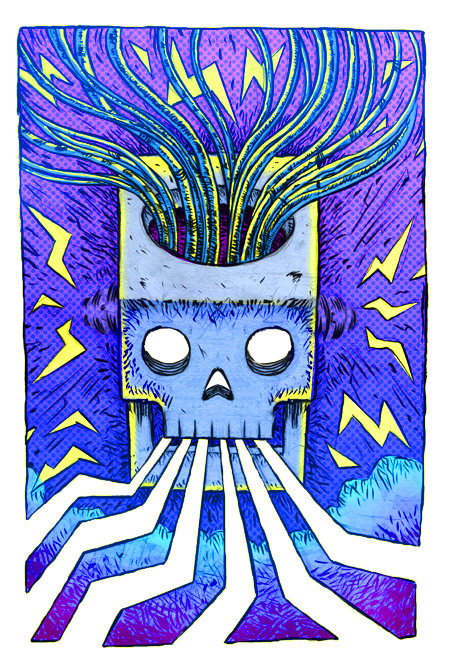
\includegraphics[scale=0.2]{images/io.jpg}}}%
  \texttt{%
    \visible<2->{\syncomment{-- Compile-Zeit-Fehler!}} \\
    \synKey{let}\ x \synSym{=}\ getLine \\
    \synKey{in}\ print (x \synOp{++}\ x)
  }

  \vspace{1em}
  vs.
  \vspace{1em}

  \texttt{%
    \visible<2->{\syncomment{-- Compile-Zeit-Fehler!}} \\
    print (getLine \synOp{++}\ getLine)
  }

  \pause
  \pause
  \vfill
  \begin{itemize}
    \item Aktionen $\neq$ Werte
    \item \texttt{getLine \synSym{::}\ \synType{IO}\ \synType{String}}
  \end{itemize}
}

\subsection[Beispiele]{Erste Beispiele: Aufsummieren und Quicksort}
\frame[t]{\frametitle{Beispiel: Aufsummieren}
  \floatbox{-210}{195}{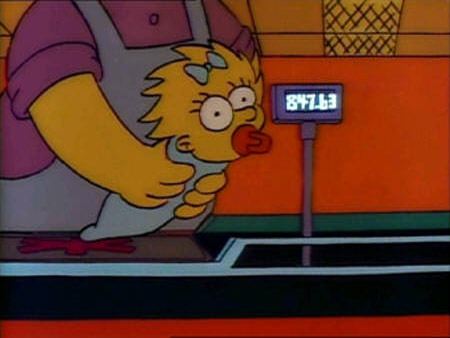
\includegraphics[scale=0.35]{images/kasse.jpg}}%
  \texttt{%
    sum []\ \ \ \ \ \synSym{=}\ 0 \\
    sum (x\synSym{:}xs) \synSym{=}\ x \synOp{+}\ sum xs
  }

  \pause\vfill
  Beispielauswertung: \\
  \texttt{%
    \ \ \ sum [\synLit{1},\synLit{2},\synLit{3}] \\
    == \synLit{1}\ \synOp{+}\ sum [\synLit{2},\synLit{3}] \\
    == \synLit{1}\ \synOp{+}\ (\synLit{2}\ \synOp{+}\ sum [\synLit{3}]) \\
    == \synLit{1}\ \synOp{+}\ (\synLit{2}\ \synOp{+}\ (\synLit{3}\ \synOp{+}\ sum [])) \\
    == \synLit{1}\ \synOp{+}\ (\synLit{2}\ \synOp{+}\ (\synLit{3}\ \synOp{+}\ \synLit{0})) \\
    == \synLit{6}
  }
}

\frame[t]{\frametitle{Beispiel: Quicksort}
  \floatbox{-230}{175}{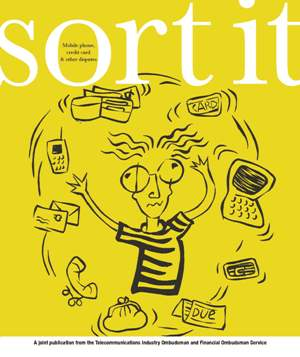
\includegraphics[scale=0.7]{images/sort.jpg}}%
  \vspace{\topskip}%
  \begin{minipage}{20cm}
    \texttt{%
      qsort []\ \ \ \ \ \synSym{=}\ [] \\
      qsort (x\synSym{:}xs) \synSym{=} \\
      \phantom{ }\ \ \ qsort kleinere \synOp{++}\ [x] \synOp{++}\ qsort groessere \\
      \phantom{ }\ \ \ \synKey{where} \\
      \phantom{ }\ \ \ kleinere\ \ \synSym{=}\ [ y \synSym{|}\ y \synSym{<-}\ xs, y \synOp{<}\ \ x ] \\
      \phantom{ }\ \ \ groessere \synSym{=}\ [ y \synSym{|}\ y \synSym{<-}\ xs, y \synOp{>=}\ x ]
    }
  \end{minipage}
}

\section{Typsystem}
\subsection{Grundtypen}
\frame[t]{\frametitle{Werte und Typen}
  \floatbox{-250}{35}{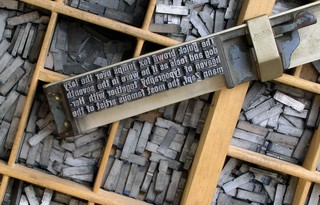
\includegraphics[scale=0.25]{images/types.jpg}}%
  \newcommand{\hatTyp}{\texttt{\synSym{::}}}%
  \vspace{-2em}%
  \begin{tabbing}
    \texttt{"Hallo, Welt!123333"} \= \hatTyp\ \= \kill
    \texttt{\synLit{"Hallo, Welt!"}} \> \hatTyp \> \texttt{\synType{String}} \\
    \texttt{\synLit{True}} \> \hatTyp \> \texttt{\synType{Bool}} \\
    \\
    \texttt{[\synLit{'A'}, \synLit{'B'}, \synLit{'C'}]} \> \hatTyp \> \texttt{[\synType{Char}]} \\
    \texttt{[[\synLit{1},\synLit{2}], [\synLit{3}], []]} \> \hatTyp \> \texttt{[[\synType{Integer}]]} \\
    \\
    \texttt{head}, \texttt{last} \> \hatTyp \> \texttt{[a] \synSym{->}\ a} \\
    \texttt{\syncomment{-- Bsp.:}\ head [\synLit{1},\synLit{2},\synLit{3}] == \synLit{1}} \\
    \texttt{\ \ \ \ \ \ \ \ \ last [\synLit{1},\synLit{2},\synLit{3}] == \synLit{3}} \\
    \\
    \texttt{init}, \texttt{tail} \> \hatTyp \> \texttt{[a] \synSym{->}\ a} \\
    \texttt{\syncomment{-- Bsp.:}\ init [\synLit{1},\synLit{2},\synLit{3}] == [\synLit{1},\synLit{2}]} \\
    \texttt{\ \ \ \ \ \ \ \ \ tail [\synLit{1},\synLit{2},\synLit{3}] == [\synLit{2},\synLit{3}]}
  \end{tabbing}
}

\subsection{Typerschließung}
\newcommand{\unhappy}{{\setlength{\tabcolsep}{0pt}\footnotesize\begin{tabular}c.\thinspace.\\[-1ex]\texttt{\char'015}\\[-1.1em]$\frown$\\[ -1.5em]\large$\bigcirc$\end{tabular}}}
\frame[plain]{\begin{center}
  \Huge java.io.InputStreamReader

  \vspace{-1em}
  \scalebox{8}{\unhappy}
\end{center}}

\frame[t]{\frametitle{Automatische Typerschließung}
  \floatbox{-170}{190}{
\includegraphics[scale=0.4]{images/katze.jpg}}%
  Automatische Erschließung nicht angegebener Typen durch den Compiler

  \texttt{%
    \ \\
    \visible<2->{%
      greet \synSym{::}\ \synType{String}\ \synSym{->}\ \synType{String}
    } \\
    greet name \synSym{=}\ \synLit{"Hallo "}\ \synOp{++}\ name \synOp{++}\ \synLit{"!"} \\
    \ \\
    \visible<4->{%
      dup \synSym{::}\ [a] \synSym{->}\ [a]
    } \\
    \visible<3->{%
      dup xs \synSym{=}\ xs \synOp{++}\ xs \\
      \syncomment{-- Bsp.:} \\
      \syncomment{\ \ \ dup [1,2,3] ==} \\
      \syncomment{\ \ \ [1,2,3,1,2,3]}
    }
  }
}

\subsection{Typklassen}
\frame[t]{\frametitle{Typklassen}
  \texttt{%
    \visible<2->{%
      add37 \synSym{::}\ \visible<3->{\colorbox{backblue}{(Num a) =>}} a \synSym{->}\ a
    } \\
    add37 x \synSym{=}\ x \synOp{+}\ 37 \\
    \syncomment{-- Bsp.: add37 5 == 42} \\
    \ \\
    \visible<5->{%
      min \synSym{::}\ \colorbox{backblue}{(Ord a) =>} a \synSym{->}\ a \synSym{->}\ a
    } \\
    \visible<4->{%
      min x y \synSym{=}\ \synKey{if}\ x \synOp{<=}\ y \synKey{then}\ x \synKey{else}\ y \\
      \syncomment{-- Bsp.: min 19 17 == 17}
    }
  }

  \pause\pause\pause\pause\pause
  \vfill
  \begin{itemize}
    \item Typklassen als Schnittstellen
    \item
      \texttt{%
        \synKey{class}\ \synType{Num}\ a \synKey{where} \\
        \ \ \ \ \synOp{(+)}\ \synSym{::}\ a \synSym{->}\ a \synSym{->}\ a \\
        \ \ \ \ \synOp{(-)}\ \synSym{::}\ a \synSym{->}\ a \synSym{->}\ a \\
        \ \ \ \ \synOp{(*)}\ \synSym{::}\ a \synSym{->}\ a \synSym{->}\ a \\
        \ \ \ \ \ldots
      }
  \end{itemize}
}

\subsection{Aktionstypen}
\frame[t]{\frametitle{Typen von Ein-/Ausgabe-Operationen}
  \newcommand{\hatTyp}{\texttt{\synSym{::}}}
  \begin{tabbing}
    \texttt{readFile} \= \hatTyp\ \= \kill
    \texttt{getLine} \> \hatTyp \> \texttt{\colorbox{backblue}{\synType{IO}}\ \synType{String}} \\
    \texttt{putStr}  \> \hatTyp \> \texttt{\synType{String}\ \synSym{->}\ \colorbox{backblue}{\synType{IO}}\ ()} \\
    \texttt{readFile} \> \hatTyp \> \texttt{\synType{FilePath}\ \synSym{->}\ \colorbox{backblue}{\synType{IO}}\ \synType{String}}
  \end{tabbing}

  \pause
  \vfill
  \setlength{\columnsep}{45pt}%
  \begin{multicols*}{2}
    \texttt{%
      main \synSym{::}\ \colorbox{backblue}{\synType{IO}}\ () \\
      main \synSym{=}\ \synKey{do} \\
      \ \ \ \ x \synSym{<-}\ getLine \\
      \ \ \ \ print (x \synOp{++}\ x) 
    }

    \columnbreak

    \texttt{%
      main \synSym{::}\ \colorbox{backblue}{\synType{IO}}\ () \\
      main \synSym{=}\ \synKey{do} \\
      \ \ \ \ x \synSym{<-}\ getLine \\
      \ \ \ \ y \synSym{<-}\ getLine \\
      \ \ \ \ print (x \synOp{++}\ y) 
    }
  \end{multicols*}
}

\frame[plain]{\begin{center}
  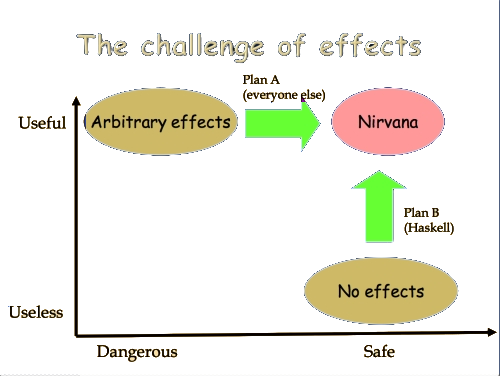
\includegraphics[scale=0.6]{images/effects.png}

  Grafik gestohlen von: Simon Peyton Jones
\end{center}}

\section[Weiteres]{Weitere Fähigkeiten}
\subsection[Parser]{Parser-Aktionen}
\frame[t]{\frametitle{Parser-Aktionen}
  \floatbox{-250}{190}{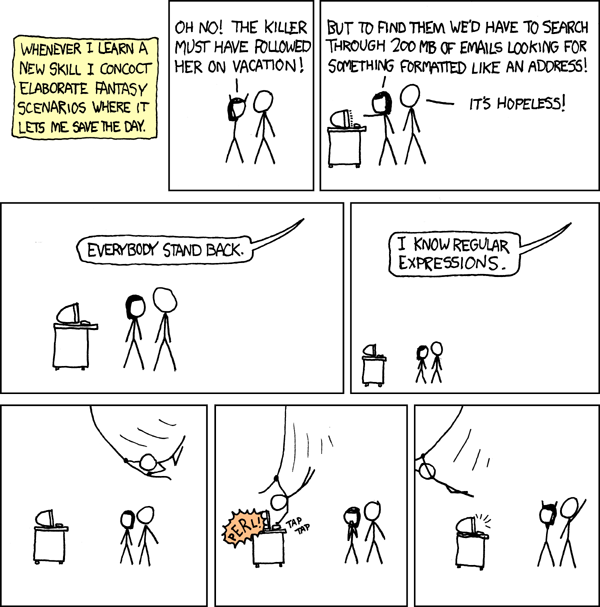
\includegraphics[scale=0.13]{images/regex.png}}%
  \texttt{%
    perlBezeichner \synSym{::}\ \synType{Parser}\ \synType{String} \\
    perlBezeichner \synSym{=}\ \synKey{do} \\
    \ \ \ \ sigil \synSym{<-}\ oneOf \synLit{"\$@\%\&"} \\
    \ \ \ \ name\ \ \synSym{<-}\ many alphaNum \\
    \ \ \ \ return (sigil \synOp{:}\ name)
  }

  \vfill
  Dabei verwendete Funktionen aus Parser-Bibliothek:
  \newcommand{\hatTyp}{\texttt{\synSym{::}}}
  \begin{tabbing}
    \texttt{alphaNum} \= \hatTyp\ \= \kill
    \texttt{oneOf} \> \hatTyp \> \texttt{[\synType{Char}] \synSym{->}\ \synType{Parser}\ \synType{Char}} \\
    \texttt{alphaNum} \> \hatTyp \> \texttt{\synType{Parser}\ \synType{Char}} \\
    \texttt{many} \> \hatTyp \> \texttt{\synType{Parser}\ a \synSym{->}\ \synType{Parser}\ [a]}
  \end{tabbing}
}

\subsection[Laziness]{Bedarfsauswertung}
\frame[t]{\frametitle{Bedarfsauswertung}
  \floatbox{-210}{195}{
\includegraphics[scale=0.2]{images/lazy.jpg}}%
  \texttt{%
    main \synSym{=}\ \synKey{do} \\
    \ \ \ \ daten \synSym{<-}\ readFile \synLit{"große-datei.txt"} \\
    \only<1>{\ \ \ \ print (lines daten \synOp{!!}\ 99)}
    \only<2->{\ \ \ \ print \synOp{\$}\ lines daten \synOp{!!}\ 99}
  }

  \pause\pause
  \vfill
  \begin{itemize}
    \item Auswertung von Ausdrücken erst dann, wenn Ergebnisse wirklich benötigt
    \item Somit Fähigkeit für \\
          unendliche Datenstrukturen: \\
          Potenzreihen, Zeitreihen, \\
          Entscheidungsbäume, \ldots
  \end{itemize}
}

\frame[t]{\frametitle{Bedarfsauswertung}
  \floatbox{-210}{150}{
\includegraphics[scale=0.2]{images/lazy.jpg}}%
  \begin{minipage}{20cm}
    \texttt{%
      natürlicheZahlen \synSym{::}\ [\synType{Integer}] \\
      natürlicheZahlen \synSym{=}\ [\synLit{1}..] \\
      \ \\
      \pause
      ungeradeZahlen \synSym{::}\ [\synType{Integer}] \\
      ungeradeZahlen \synSym{=}\ filter odd [\synLit{1}..] \\
      \ \\
      \pause
      fibs \synSym{::}\ [\synType{Integer}] \\
      fibs \synSym{=}\ \synLit{0}\ \synOp{:}\ \synLit{1}\ \synOp{:}\ zipWith\ \synOp{(+)}\ fibs (tail fibs)
    }
  \end{minipage}
}

\subsection[Datentypen]{Benutzerdefinierte Datentypen}
\frame[t]{\frametitle{Benutzerdefinierte Datentypen}
  \floatbox{-220}{190}{\scalebox{0.7}{\input{images/baum.pspdftex}}}%
  \texttt{%
    \synKey{data}\ \synType{Tree}\ = Leaf \synType{Int}\ | Fork \synType{Tree}\ \synType{Tree}
  }
  Konstruktoren: \\
  \texttt{Leaf \synSym{::}\, Int \synSym{->}\ Tree} und \\
  \texttt{Fork \synSym{::}\, Tree \synSym{->}\ Tree \synSym{->}\ Tree}

  \vfill
  \pause
  \texttt{%
    beispielBaum \synSym{=}\ Fork \\
    \ \ \ \ (Fork (Leaf \synLit{17}) (Leaf \synLit{37}))\\
    \ \ \ \ (Fork\\
    \ \ \ \ \ \ \ \ (Fork (Leaf \synLit{42}) (Leaf \synLit{0}))\\
    \ \ \ \ \ \ \ \ (Leaf \synLit{41}))
  }

  \vfill
  \pause
  \texttt{%
    komischerBaum \synSym{=}\ Fork \\
    \ \ \ \ (Fork (Leaf \synLit{23}) komischerBaum)
  }
}

\frame[t]{\frametitle{Benutzerdefinierte Datentypen (Forts.)}
  \floatbox{-223}{75}{\scalebox{0.7}{\input{images/baum.pspdftex}}}%
  \hspace*{-1em}\begin{minipage}{20cm}
  \texttt{%
    \only<1>{%
      \synKey{data}\ \synType{Tree}\ \ \ = Leaf \synType{Int}\ | Fork \synType{Tree}\ \synType{Tree}
    }%
    \only<2->{\sout{%
      \synKey{data}\ \synType{Tree}\ \ \ = Leaf \synType{Int}\ | Fork \synType{Tree}\ \synType{Tree}
    }} \\
    \ \\
    \pause
    \synKey{data}\ \synType{Tree}\ a = Leaf a \ \ | Fork (\synType{Tree}\ a) (\synType{Tree}\ a)
    \pause
    \ \\
    \ \\
    size \synSym{::}\ \synType{Tree}\ a \synSym{->}\ \synType{Integer} \\
    size (Leaf \symbol{95})\ \ \ \ \ \ \ \ \ \ \ \ \synSym{=}\ \synLit{1} \\
    size (Fork links rechts) \synSym{=}\\
    \phantom{ }\ \ \ size links \synOp{+}\ size rechts
    \ \\
    \ \\
    \pause
    inorder \synSym{:}\ \synType{Tree}\ a \synSym{->}\ [a] \\
    inorder (Leaf x)\ \ \ \ \ \ \ \ \ \ \ \  \synSym{=}\ [x] \\
    inorder (Fork links rechts) \synSym{=} \\
    \phantom{ }\ \ \ inorder links \synOp{++}\ inorder rechts
  }
  \end{minipage}
}

\subsection{QuickCheck}
\frame[t]{\frametitle{QuickCheck}
  \floatbox{-253}{200}{
\includegraphics[scale=0.2]{images/pruefung.jpg}}%
  \texttt{%
    \syncomment{\# Perl} \\
    \synfunc{is}(\synfunc{sqrt}(0), \ 0, \synstr{"{}sqrt(0) ist ok"}); \\
    \synfunc{is}(\synfunc{sqrt}(1), \ 1, \synstr{"{}sqrt(1) ist ok"}); \\
    \synfunc{is}(\synfunc{sqrt}(4), \ 2, \synstr{"{}sqrt(4) ist ok"}); \\
    \synfunc{is}(\synfunc{sqrt}(9), \ 3, \synstr{"{}sqrt(9) ist ok"}); \\
    \synfunc{is}(\synfunc{sqrt}(16), 4,  \synstr{"{}sqrt(16) ist ok"}); \\
    \ldots;\ \ \syncomment{\# ??}
  }

  \vfill
  \pause
  \texttt{%
    \syncomment{-- Haskell mit QuickCheck} \\
    propSqrt \synSym{::}\ \synType{Double}\ \synSym{->}\ \synType{Bool} \\
    propSqrt x \synSym{=}\ sqrt (x \synOp{*}\ x) \synOp{==}\ x
  }
}

\frame[t]{\frametitle{QuickCheck (Forts.)}
  \floatbox{-253}{200}{
\includegraphics[scale=0.2]{images/pruefung.jpg}}%
  \texttt{%
    propSqrt \synSym{::}\ \synType{Double}\ \synSym{->}\ \synType{Bool} \\
    propSqrt x \synSym{=}\ sqrt (x \synOp{*}\ x) \synOp{==}\ x \\
    \ \\
    ghci> quickCheck propSqrt \\
    Falsifiable, after 6 tests: \\
    -0.25
  }
  \pause

  \vfill
  \texttt{%
    propSqrt' \synSym{::}\ \synType{Double}\ \synSym{->}\ \synType{Bool} \\
    propSqrt' x \synSym{=}\ sqrt (x \synOp{*}\ x) \synOp{==}\ \colorbox{backblue}{abs} x \\
    \ \\
    ghci> quickCheck propSqrt' \\
    OK, passed 100 tests.
  }
}

\frame[t]{\frametitle{QuickCheck (Forts.)}
  \floatbox{-253}{200}{
\includegraphics[scale=0.2]{images/pruefung.jpg}}%
  \vspace{-\topsep}%
  \begin{itemize}
    \item Überprüfung durch zufällig generierte Stichproben
    \item \texttt{%
      \synKey{class}\ \synType{Arbitrary}\ a \synKey{where} \\
      \ \ \ \ arbitrary \synSym{::}\ \synType{Gen}\ a
    }
    \item Instanzen von \texttt{\synType{Arbitrary}} nicht nur für
          primitive, sondern automatisch auch für zusammengesetzte Typen
  \end{itemize}
  \vfill

  \pause
  \vfill
  \texttt{%
    \synKey{import}\ Data.Char \\
    kleinbuchstabe \synSym{::}\ \synType{Gen}\ \synType{Char} \\
    kleinbuchstabe \synSym{=}\ \synKey{do} \\
    \ \ \ \ c \synSym{<-}\ arbitrary \\
    \ \ \ \ return (toUpper c)
  }
}

\subsection[FFI]{Foreign Function Interface}
\frame[t]{\frametitle{Foreign Function Interface}
  \texttt{%
    \syncomment{\{-\# INCLUDE <math.h> \#-\}} \\
    foreign \synKey{import}\ ccall unsafe "{}sin"{}\\
    \ \ \ \ c\_{}sin \synSym{::}\ \synType{CDouble}\ \synSym{->}\ \synType{CDouble} \\
  }

  \vfill
  \begin{itemize}
    \item Einbindung von (C-)Bibliotheken
    \item Keine besondere Handhabung der importierten Funktionen
    \item Callbacks aus dem C-Code heraus möglich
  \end{itemize}
}

\section{Gemeinschaft}
\subsection{Hackage}
\frame[t]{\frametitle{Paketarchiv Hackage}
  \begin{itemize}
    \item Entstehung 2007, mittlerweile $2300^+$ Pakete
    \item Installationswerkzeug cabal-install
  \end{itemize}

  \vspace{-0.6em}
  \begin{center}
    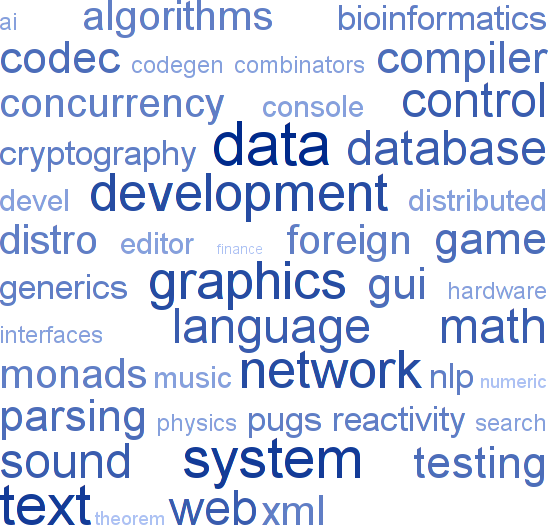
\includegraphics[scale=0.35]{images/cloud.png}
  \end{center}
}

\subsection{Größere Anwendungen}
\frame[t]{\frametitle{Größere Anwendungen}
  \begin{itemize}
    \item Glasgow Haskell Compiler (GHC)
    \item Verteiltes Versionskontrollsystem: Darcs
    \item Fenstermanager: xmonad
    \item Perl-6-Prototyp: Pugs
    \item Sprache für kryptographische Algorithmen: Cryptol
    \item Benchmarkbibliothek: Criterion
  \end{itemize}

  \begin{center}
    \hfill
    
\includegraphics[scale=0.9]{images/darcs.png}
    \hfill
    
\includegraphics{images/xmonad.png}
    \hfill
    
\includegraphics[scale=0.8]{images/cryptol.png}
    \hfill
  \end{center}
}

\subsection{Einstiegspunkte}
\frame[t]{
  \begin{itemize}
    \item \url{http://haskell.org/}
          \vspace{2\itemsep}
    \item zum Herumspielen im Browser: \\
          \url{http://tryhaskell.org/}
    \item interaktive Haskell-Shell: \\
          \texttt{\$ apt-get install ghc6} \\
          \texttt{\$ ghci}
          \vspace{2\itemsep}
    \item \texttt{\#haskell} auf Freenode
    \item \url{http://planet.haskell.org/}
          \vfill
    \item Teile dieses Vortrags inspiriert von einem Vortrag von
          Audrey Tang: \\
          \url{http://feather.perl6.nl/~audreyt/osdc/haskell.xul}
  \end{itemize}
}

\frame{\begin{center}
  \floatbox{-165}{130}{
\includegraphics[scale=0.5]{images/thankyou.png}}%
  
\includegraphics[scale=0.7]{images/luga.png}
  \vspace{3em}

  \Huge \syncool{-- Haskell --}
\end{center}}

\appendix
\frame{
  \floatbox{-200}{180}{
\includegraphics[scale=0.25]{images/present.png}}%
  \begin{center}\Huge Bonus-Folien\end{center}

  \tableofcontents
}

\section[Fehlende Werte]{Umgang mit fehlenden Werten}
\frame[t]{\frametitle{Umgang mit fehlenden Werten}
  \floatbox{-260}{120}{
\includegraphics[scale=0.25]{images/bug.png}}%
  \vspace{-\topsep}%
  \begin{itemize}
    \item "`Null References: The Billion Dollar Mistake`` (Tony Hoare)
    \item In Haskell: Explizite Kennzeichnung von möglicherweise fehlenden
          Werten durch Maybe-Typen
  \end{itemize}
  \vfill

  \texttt{%
    \synKey{data}\ \synType{Maybe}\ a \synSym{=}\ Nothing \synSym{|}\ Just a \\
    \ \\
    lookupFarbe \synSym{::}\ \synType{String}\ \synSym{->}\ \colorbox{backblue}{\synType{Maybe}} \synType{Color} \\
    \syncomment{-- Bsp.:} \\
    \syncomment{\ \ \ lookupFarbe "{}Simpsons"{} == Just YELLOW} \\
    \syncomment{\ \ \ lookupFarbe "{}Simqsons"{} == Nothing} \\
  }
}

\frame[t]{\frametitle{Maybe-Ketten}
  Anwendbarkeit des syntaktischen Zuckers für Aktionstypen für Maybe:
  \vfill

  \texttt{%
    berechneA \synSym{::}\ \synType{Integer}\ \ \synSym{->}\ \synType{Maybe}\ \synType{String} \\
    berechneB \synSym{::}\ \synType{Integer}\ \ \synSym{->}\ \synType{Maybe}\ [\synType{Double}] \\
    berechneC \synSym{::}\ [\synType{Double}]\ \synSym{->}\ \synType{Maybe}\ \synType{String} \\
    \ \\
    berechne \synSym{::}\ \synType{Integer}\ \synSym{->}\ \synType{Maybe}\ \synType{String} \\
    berechne x \synSym{=}\ \synKey{do} \\
    \ \ \ \ teil1\ \ \synSym{<-}\ berechneA x \\
    \ \ \ \ teil2\ \ \synSym{<-}\ berechneB x \\
    \ \ \ \ teil2'   \synSym{<-}\ berechneC teil2 \\
    \ \ \ \ return (teil1 \synOp{++}\ teil2)
  }
}

\section{Bildquellen}
\frame[t]{\frametitle{Bildquellen}
  \tiny
  \begin{itemize}
    \item \url{http://learnyouahaskell.com/splash.png}
    \item \url{http://save-endo.cs.uu.nl/target.png}
    \item \url{http://media.nokrev.com/junk/haskell-logos/logo7.png}
    \item \url{http://theleftwinger.files.wordpress.com/2010/01/lazy.jpg}
    \item \url{http://www.nataliedee.com/093009/death-is-a-side-effect-of-most-things.jpg}
    \item \url{http://www.sketchybeast.com/wp-content/uploads/2007/12/input_output.jpg}
    \item \url{http://www.homemortgagerates.us/variable-rates-636.jpg}
    \item \url{http://upload.wikimedia.org/wikipedia/commons/c/c6/Metal_movable_type_edit.jpg}
    \item \url{http://imgs.xkcd.com/comics/regular_expressions.png}
    \item \url{http://wordaligned.org/images/the-challenge-of-effects.jpg}
    \item \url{http://www.lakehousecreations.com/images/ThankYou/Thank\%20You\%202003\%20(12).jpg}
    \item \url{http://i.ehow.com/images/a04/8i/g0/show-real-smile-photographs-800X800.jpg}
    \item \url{http://www.galois.com/~dons/images/cloud.png}
    \item \url{http://www.sopaed-lern.uni-wuerzburg.de/uploads/pics/Pruefung.jpg}
    \item \url{http://perl.plover.com/yak/presentation/samples/present.gif}
    \item \url{http://upload.wikimedia.org/wikipedia/commons/7/7d/Bug.png}
    \item \url{http://www.fos.org.au/custom/files/media/sort_it_cover_300.jpg}
    \item \url{http://www.simpsonsline.com/rb/fakten/vorspann/02_kasse.jpg}
    \item \url{http://www.darcs.net/logos/logo.png}
    \item \url{http://xmonad.org/images/logo.png}
    \item \url{http://www.galois.com/files/Cryptol/Cryptol_logo_image.png}
    \item \url{http://www.luga.de/LUGA_Logo}
  \end{itemize}
}

\end{document}
